% This is a basic Math Paper

\documentclass[11pt]{article}

% Preamble

\usepackage[margin=1in]{geometry}
\usepackage{amsfonts, amsmath, amssymb}
\usepackage{fancyhdr, float, graphicx}
\usepackage[utf8]{inputenc} % Required for inputting international characters
\usepackage[T1]{fontenc} % Output font encoding for international characters
\usepackage{fouriernc} % Use the New Century Schoolbook font
\usepackage[nottoc, notlot, notlof]{tocbibind}
\usepackage{url}
\usepackage{placeins}
\usepackage{multirow}
% Header and Footer
\pagestyle{fancy}
\fancyhead{}
\fancyfoot{}
\fancyhead[L]{\textit{\Large{Experiment 5}}}
%\fancyhead[R]{\textit{something}}
\fancyfoot[C]{\thepage}
\renewcommand{\footrulewidth}{1pt}



% Other Doc Editing
% \parindent 0ex
%\renewcommand{\baselinestretch}{1.5}

\begin{document}
	
	\begin{titlepage} 
		\centering 
		
		%---------------------------NAMES-------------------------------
		
		\huge\textsc{
			MIT World Peace University
		}\\
	
		\vspace{0.75\baselineskip} % space after Uni Name
		
		\LARGE{
			Physics\\
			First Year B. Tech, Trimester 3\\
			Academic Year 2021-22
		}
		
		\vfill % space after Sub Name
		
		%--------------------------TITLE-------------------------------
		
		\rule{\textwidth}{1.6pt}\vspace*{-\baselineskip}\vspace*{2pt}
		\rule{\textwidth}{0.6pt}
		\vspace{0.75\baselineskip} % Whitespace above the title
		
		
		
		\huge{\textsc{
			Measuring width of an ultra-thin
			slit, diameter of an ultra-thin wire and counting number of slits in diffraction
			grating using He Ne laser
			}} \\
		
		
		
		\vspace{0.5\baselineskip} % Whitespace below the title
		\rule{\textwidth}{0.6pt}\vspace*{-\baselineskip}\vspace*{2.8pt}
		\rule{\textwidth}{1.6pt}
		
		\vspace{1\baselineskip} % Whitespace after the title block

		%--------------------------SUBTITLE --------------------------	
			
		\LARGE\textsc{
			Experiment No. 5
		} % Subtitle or further description
		\vfill
		
		%--------------------------AUTHOR-------------------------------
		
		Prepared By
		\vspace{0.5\baselineskip} % Whitespace before the editors
		
		\Large{
			109054. Krishnaraj Thadesar
			
			Division 9 Batch I3
		}
		
		
		\vspace{0.5\baselineskip} % Whitespace below the editor list
		\today

	\end{titlepage}

	\begin{center}
	{\Large Pledge}\\
	\vspace{0.5cm}
	I solemnly affirm that I am presenting this journal based on my own experimental work. I have neither copied the observations, calculations, graphs and results from others nor given it to others for copying.\\
		\end{center}
	
	\vspace{0.5cm}
	
    \begin{flushright}
	{\large Signature of the student}\\
	\vspace{1cm}
	 \end{flushright}
	
	

	\section{Aim}
	\noindent
	Using He-Ne Laser to: 
	 \begin{enumerate}
		 \item Measure width of a narrow slit
   \item Measure diameter of a thin wire. 
   \item Counting the number of slits in a diffraction grating. 
	 \end{enumerate}
	
	\section{Apparatus}


		\begin{enumerate}
			\item He-Ne Laser
			\item A narrow slit
   \item a thin wire. 
   \item Diffraction Grating
   \item optical bench with stands to moutn slit, wire and grating
   \item Screen
   \item Scale
		\end{enumerate}


	\section{Significance of the Experiment}
\textit{This experiment demonstrates three out of several applications
of laser. The conventional techniques for measuring the width of narrow slits and thin wires are
tedious and error prone. Laser provides an easy and accurate method to measure these
quantities. Secondly, counting enormously large number of slits in the grating using any other
method is almost impossible, however, laser makes it possible}
	
	
	\section{Theory}
	Laser is an extremely coherent, monochromatic, directional, focusable, polarized and
	powerful light. These extraordinary features make it greatly applicable in day-to-day life, science
	and technology. A few notable applications of laser include medical diagnosis and treatments,
	fiber optic communications, CD-ROMS, CD players, laser printers, defense, cutting, welding,
	drilling, surveying, aligning etc.\\

	Laser is produced due to stimulated radiation; a process where a resonating photon
stimulates the de-excitation of an excited atom. This results in to emission of two coherent
photons, which are identical in all respects. These photons further stimulate the de-excitation of
other excited atoms and this continues to generate an avalanche of coherent photons. For
stimulated emission to take over spontaneous emission and stimulated absorption, a few
conditions are necessary. These are availability of metastable state (life time = 10-3 sec),
population inversion (greater number of atoms in metastable state than in lower energy state) and
enough number of photons in the cavity (mirrors).
	\begin{figure}[H]
		\centering
		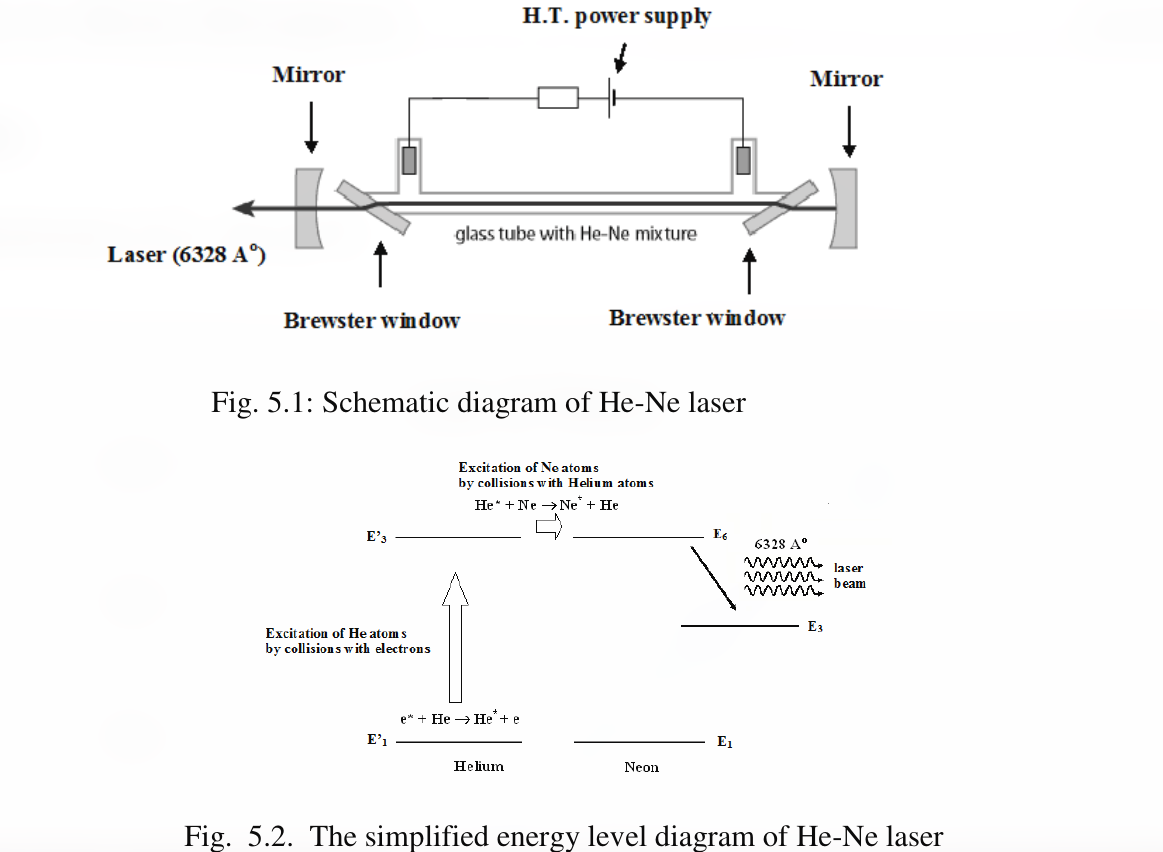
\includegraphics[scale=0.5]{1.png}
		\label{it}
	\end{figure}
	
\subsection{He Ne Laser}
He-Ne laser is a low power, continuous gas laser, which is used in supermarket scanners, student
laboratories and holography. The active system is neon, which is pumped electronically via
helium in a resonant cavity made of discharge tube (Fig. 5.1) . The main lasing occurs in neon
between the levels E6 (metastable) and E3 which produces an intense coherent beam of red color
(wavelength 6328o). (refer Fig 5.2). The population of photons necessary for stimulated emission
is maintained by mirrors (one is semitransparent) on both sides. Brewseter windows are used to
polarize the laser light.


\subsection{Measuring width of a narrow slit}

	Consider a narrow slit of width a exposed to a laser of wavelength $\lambda$. The laser is diffracted
	through the slit and a diffraction pattern, as shown in Fig 6.1 is produced. It consists of central
	maximum, minima and secondary maxima. According to theory of single slit diffraction, the
	angular position, $\theta$ of the mth minimum is given by
	\begin{equation}
		a \sin\theta = m\lambda
	\end{equation}

	The central maximum is the principle image of the slit and it is bounded by 1st minima on both
	the sides. Therefore taking m = 1 and rearranging for a, Eqn 6.1 becomes

	\begin{equation}
		a = \frac{\lambda}{\sin\theta}
	\end{equation}
	\begin{figure}[H]
		\centering
		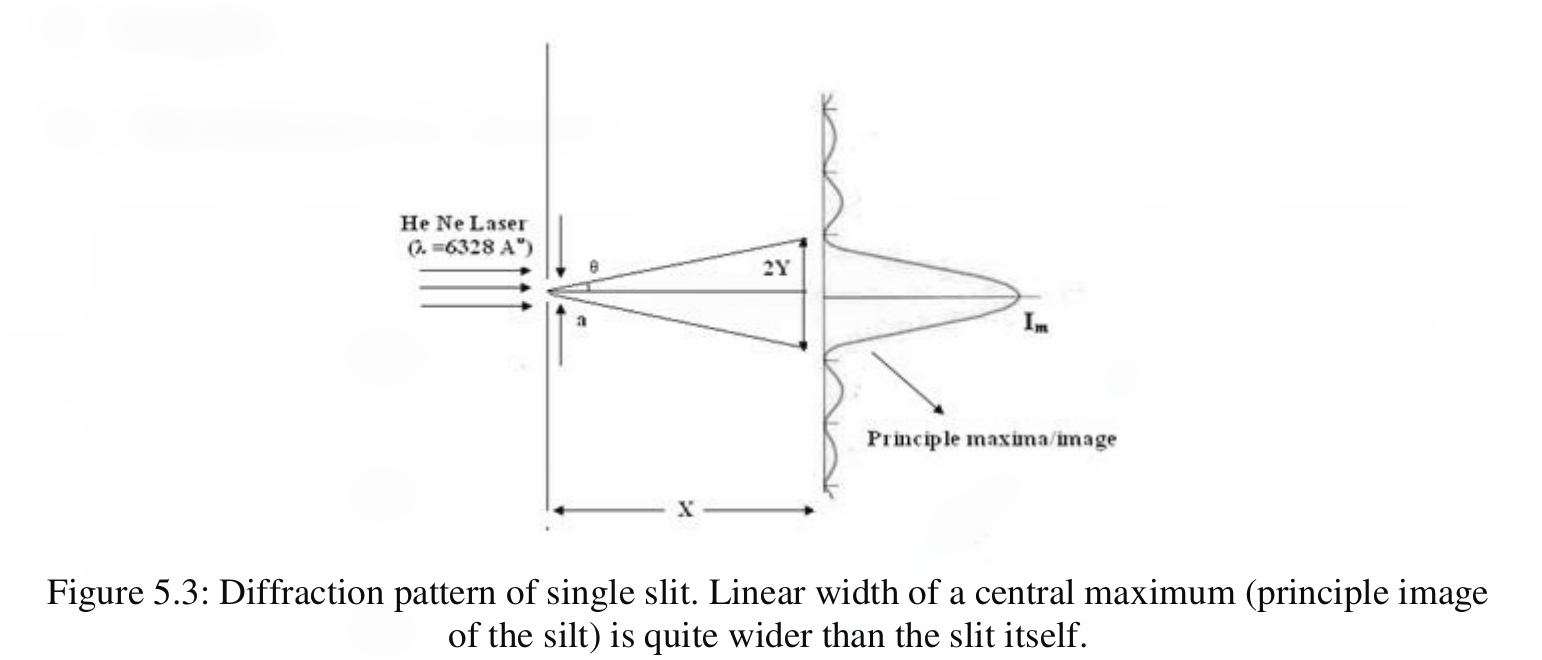
\includegraphics[scale=0.4]{2.png}
		\label{it}
	\end{figure}
	
	Thus, the width of the slit can be measured if $\lambda$ is known and $\theta$ is measured. The geometry of
the Fig 6.1 suggests that

\begin{equation}
	\tan\theta = \frac{Y}{X}
\end{equation}


where $$Y=\frac{2Y}{2} \textit{ (2Y = full linear width of the central maximum)}$$
$$ X = \textit{ distance between the slit and the screen}$$

Equations 5.1, 5.2 and 5.3 collectively indicate that narrower the slit, greater is the value of $\theta$,
thus greater is the value of 2Y. 2Y i.e. the principle image of the slit is considerably larger than
the slit itself. The relatively large value of 2Y makes its measurement easy. As against this, the
conventional techniques, which are based on direct measurements, find it more difficult to
measure the width of the slit if it is narrower.
\subsection{Measuring the diameter of a thin wire}
Consider a thin wire having diameter d exposed to a laser of wavelength $\lambda$. The wire diffracts the
light and a diffraction pattern similar to as shown in the Fig 6.2 is observed. The diffraction
pattern consists of a central maximum surrounded by maxima of almost same intensity on the
upper and lower side. These three distinct maxima are surrounded by several secondary maxima
and minima. If x is the distance between the first maximum on upper side and the first maximum
on the lower side of the central maximum and if D is the distance between wire and screen,
then it can be shown that
\begin{equation}
	d = \frac{\lambda \times d}{x}
\end{equation}
Thus if $\lambda$ is known, and if x and D are measured then the diameter of the thin wire can be
calculated. It can be noted from Eqn 6.4 that the dependence of x on d is inverse. Thus if the
wire is thinner, then x is large and thus can be measured more conveniently. Thus laser technique
is particularly advantageous for thinner wires. On the contrary, thinner the wire, more it is
difficult to measure its diameter by using conventional techniques.
\begin{figure}[H]
	\centering
	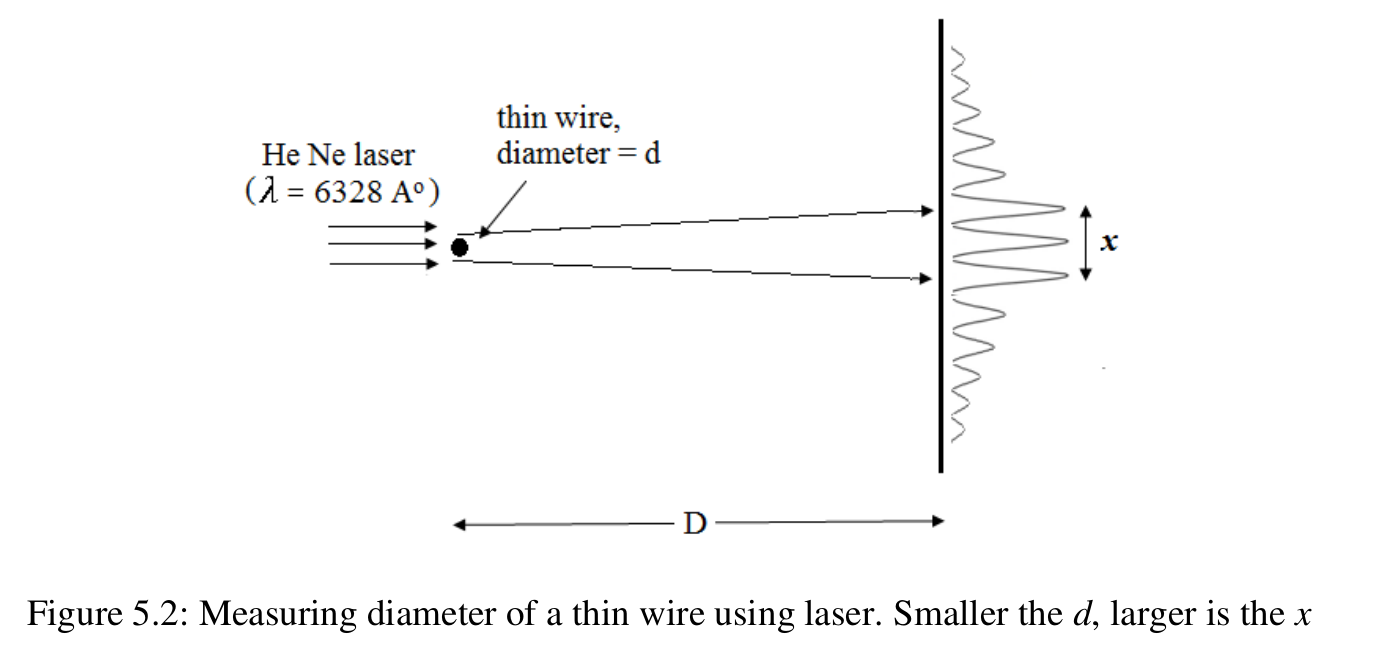
\includegraphics[scale=0.4]{3.png}
	\label{it}
\end{figure}

We know that diffraction is prohibited when the obstacle is smaller than the wavelength
of light. Thus laser cannot be used for measuring the dimensions of the slits and wires having
dimensions smaller than the wavelength of the laser. It may also be noted that if the dimensions
of the obstacle is considerably larger than the wavelength of the light then diffraction effects are
feeble. Thus the dimensions of slits and wires having size considerably larger than the
wavelength of laser cannot be measured using laser.\\
\subsection{Counting the number of slits in the diffraction grating}


Consider a monochromatic light of wavelength$\lambda$ incident on a grating having
grating element d (spacing between the slits). The light is diffracted and a diffraction pattern as
shown in Fig (6.3) is produced. According to theory of diffraction grating, the angle of
diffraction $\theta$ of a principle maxima of order m is given by

\begin{equation}
	d\sin\theta = m\lambda
\end{equation}

As seen in Fig 5.3, $\theta$ can be calculated using following relation
$$
\tan \theta=\frac{Y_{1}}{X_{1}}
$$
Where $Y_{l}=$ the distance between the central maximum and the first maximum and $X_{I}=$ distance between the grating and the screen
Thus according to eqn (5.6) if $\lambda$ and $\theta$ are substituted, then the grating element $d$ can be calculated.

If a grating consists of $N$ number slits per unit length, then it consists of $N$ number of grating elements $(d)$ per unit length. Thus
$$
d=\frac{1}{N} \Rightarrow N=\frac{1}{d}
$$
If $d$ is expressed in $\mathrm{A}^{\mathrm{o}}$, then
$$
N\left(\text { number of slits per } A^{o}\right)=\frac{1}{d\left(A^{o}\right)}, \Rightarrow N(\text { number of slits per inch })=\frac{2.54 \times 10^{8}}{d\left(A^{o}\right)}
$$
Eqn (5.9) enables us to count the number of slits in the grating even though it is very large
\begin{figure}[H]
	\centering
	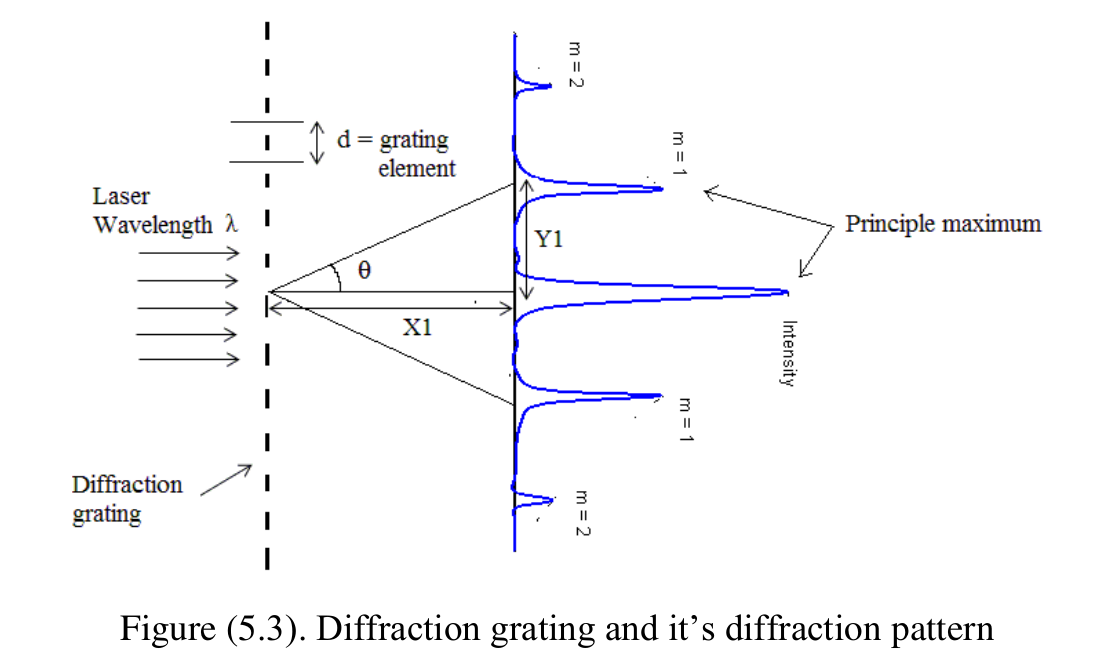
\includegraphics[scale=0.4]{4.png}
	\label{it}
\end{figure}

\clearpage
\section{Procedure}
	
\textbf{Part A. Measuring width of a narrow slit:}\\

\begin{enumerate}
	\item Make laser ON. Avoid eye contact.
	\item  Place the screen in front of the optical bench at sufficiently large distance.
	\item Mount the slit on the optical bench such that the laser is incident exactly on the slit. Align it properly so that a well-defined and distinct diffraction pattern consisting of central maximum surrounded by minima and secondary maxima is observed on the screen
	\item Measure the full width of the central maximum. This is $2 Y(\mathrm{~cm})$. Calculate $Y(\mathrm{~cm})$.
	\item Measure the distance between the slit and the screen. Let this be $X(\mathrm{~cm})$
	\item Calculate $\theta$ and the width of the slit $a_{e}(\mathrm{~mm})$ by using the procedure in table 6.1.
	\item Compare $a_{e}$ with standard width of the slit $\left(a_{s}\right)$ and calculate the percentage deviation.
	\item Tabulate all observations, calculations and results as per table $5.1$
\end{enumerate}
\noindent
\textbf{Part B: Measuring diameter of a thin wire}\\
\begin{enumerate}
	\item Fix the wire on a suitable mount. Clamp the mount on the stand. Fix the stand on the optical bench.
	\item Illuminate this wire by laser. Use trial and error method the expose the wire completely to the laser, so that a well-defined diffraction is observed on the screen. As shown in Fig (6.2), the pattern should consist of a central maximum surrounded by $1^{\text {st }}$ maxima of almost similar intensity on upper as well as lower side. These three maxima are surrounded by several secondary maxima and minima on both the sides.
	\item Measure the distance between the first maxima on the upper side and first maxima on the lower side of the central maximum. Let this be $x(\mathrm{~mm})$
	\item Measure the distance between the screen and the wire. Let this be $D(\mathrm{~mm})$.
	\item Calculate the diameter of the wire $d_{e}(\mathrm{~mm})$ by using the procedure in table $5.2$.
	\item Compare $d_{e}$ with standard $d_{s}$. Calculate the percentage deviation.
	\item Express all observations, calculations and results as per table 5.2.
\end{enumerate}
\noindent
\textbf{Part C: Counting the number of slits of a grating}
\begin{enumerate}

	\item Mount the diffraction grating on a stand. Clamp the stand on the optical bench
	\item Place laser behind the diffraction grating. Align the diffraction grating such that the laser is incident exactly perpendicularly on the grating.
	\item Place a screen in front of the grating. A well-defined diffraction pattern similar to as shown in Fig (6.3) will be observed. Only principle maxima will be observed. Secondary maxima are too weak to be observable. If the grating is sufficiently close to the screen, then central maximum, first maximum as well as second maximum will be observed.
	\item As shown in Fig (6.3), measure the distance between the first maximum and the central maximum $\left(Y_{l}\right)$ and the distance between screen and the grating $\left(X_{I}\right)$.
	\item Calculate $\theta, d\left(A^{o}\right)$ and $N_{e}$ as per the procedure given in table 5.3.
	\item Compare $N_{e}$ with standard $N_{s}$. Calculate the percentage deviation
	\item Express the observations, calculations and results as per table $5.3$

\end{enumerate}

\clearpage

\section{Observations}


\begin{figure}[H]
	\centering
	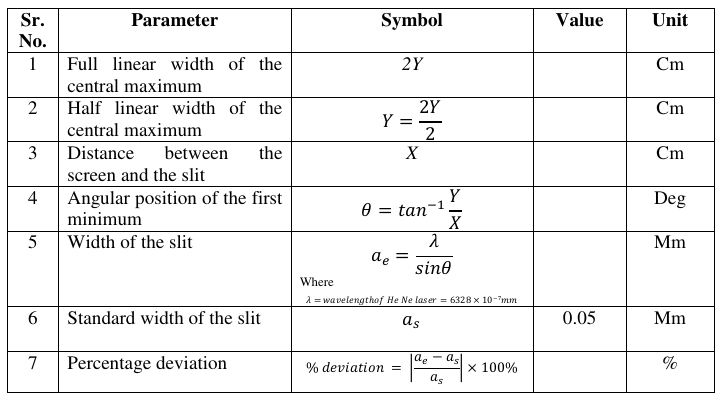
\includegraphics[scale=0.8]{widthofslit.png}
	\caption{Measuring the Width of slit}
	\label{it}
\end{figure}

\begin{figure}[H]
	\centering
	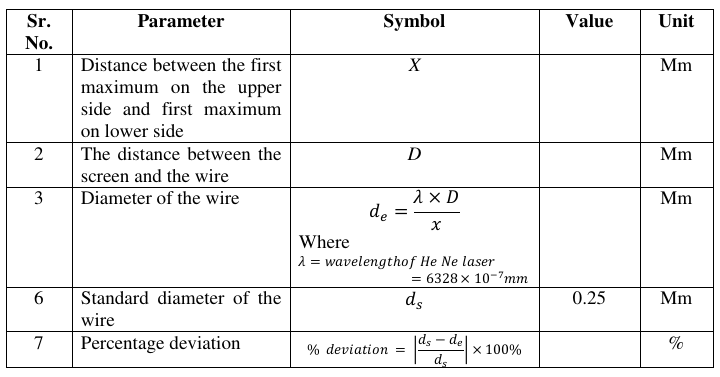
\includegraphics[scale=0.8]{diathinwire.png}
	\caption{Measuring the Diameter of thin wire}
	\label{it}
\end{figure}

\begin{figure}[H]
	\centering
	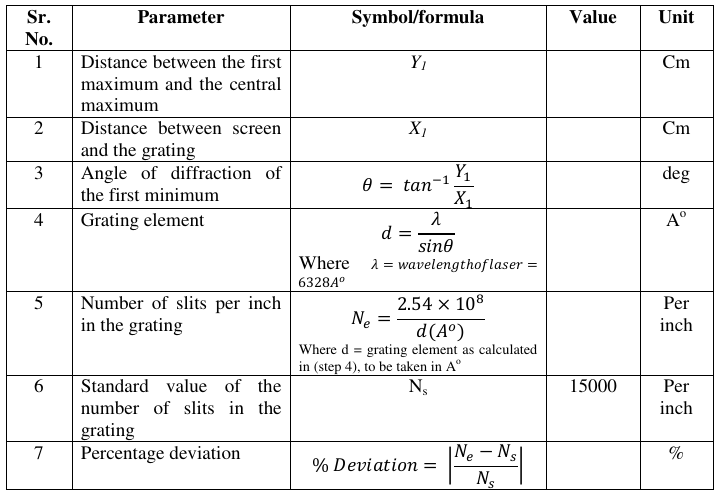
\includegraphics[scale=0.8]{noslitsgrating.png}
	\caption{Counting the number of slits in the grating}
	\label{it}
\end{figure}


\section{My Understanding of the Experiment}

This is a rather straight forward experiment, with just application of formulas, but it has proven to be
one of th most revolutionary experiments in all of physics, proving decisively the existance of light as a wave.
Replicating the Single and double slit experiment, with in this case multiple sits, and the sodium lamp with laser, gives us
a sharper interference pattern, and that makes application of the formulas easier to calculate the necessary parameter. 
Its application is therefore in places where the precise measurement of certain small quantities is essential.

\end{document}